\documentclass[12pt, a4paper]{article}% тип документа, размер шрифта
\usepackage[T2A]{fontenc}%поддержка кириллицы в ЛаТеХ
\usepackage[utf8]{inputenc}%кодировка
\usepackage[russian]{babel}%русский язык
\usepackage{mathtext}% русский текст в формулах
\usepackage{amsmath}%удобная вёрстка многострочных формул, масштабирующийся текст в формулах, формулы в рамках и др.
\usepackage{amsfonts}%поддержка ажурного и готического шрифтов — например, для записи символа {\displaystyle \mathbb {R} } \mathbb {R} 
\usepackage{amssymb}%amsfonts + несколько сотен дополнительных математических символов
\frenchspacing%запрет длинного пробела после точки
\usepackage{setspace}%возможность установки межстрочного интервала
\usepackage{indentfirst}%пакет позволяет делать в первом абзаце после заголовка абзацный отступ
\usepackage[unicode, pdftex]{hyperref}
\onehalfspacing%установка полуторного интервала по умолчанию
\usepackage{graphicx}%подключение рисунков
\graphicspath{{images/}}%путь ко всем рисункам
\usepackage{caption}
\usepackage{float}%плавающие картинки
\usepackage{tikz} % это для чудо-миллиметровки
\usepackage{pgfplots}%для построения графиков
\pgfplotsset{compat=newest, y label style={rotate=-90},  width=10 cm}%версия пакета построения графиков, ширина графиков
\usepackage{pgfplotstable}%простое рисование табличек
\usepackage{lastpage}%пакет нумерации страниц
\usepackage{comment}%возможность вставлять большие комменты
\usepackage{float}
%%%%% ПОЛЯъ
\setlength\parindent{0pt} 
\usepackage[top = 2 cm, bottom = 2 cm, left = 1.5 cm, right = 1.5 cm]{geometry}
\setlength\parindent{0pt}
%%%%% КОЛОНТИТУЛЫ
\usepackage{xcolor}
\usepackage{amsmath}
\usepackage{gensymb}
\usepackage{tikz}

\begin{document}


\subsubsection*{Гравитация. Сила тяжести.}
Начнём с самого общего закона (\textit{Закона всемирного тяготения}): любые два тела во Вселенной притягиваются друг к другу силой, которая прямо пропорциональна 
произведению их масс и обратно пропорциональна квадрату расстояния между ними. Запишем это так:
\[
F = G \,\frac{M\,m}{r^2},
\]
где
\begin{itemize}
  \item $F$ — модуль силы притяжения между двумя телами;
  \item $G$ — гравитационная постоянная, численно равная примерно $6{.}674\times10^{-11}\ \mathrm{м^3\,кг^{-1}\,с^{-2}}$;
  \item $M$ и $m$ — массы взаимодействующих тел (в килограммах);
  \item $r$ — расстояние между центрами масс этих тел (в метрах).
\end{itemize}
На практике, когда речь идёт о силе притяжения тела массы $m$ к Земле массы $M_{\oplus}$, расстояние $r$ рассчитывается от тела до центра Земли.
Это расстояние почти не меняется при движении по поверхности, поскольку Земля очень большая (её радиус составляет $\sim 6400$ км). Вводят \textit{ускорение свободного падения}
\[
g = G\,\frac{M_{\oplus}}{R_{\oplus}^2},
\]
где $R_{\oplus}$ — радиус Земли (приблизительно $6{.}37\times10^6\ \mathrm{м}$). Тогда \textit{силу тяжести} на поверхности Земли удобно записать так:
\[
F = mg.
\]
Численно $g\approx9{.}8\ \mathrm{м/с^2}$. Если тело отпустить в свободное падение, именно с таким ускорением оно будет двигаться.

\subsubsection*{Нормальная реакция опоры}
\textit{Нормальная реакция опоры} $N$ — это сила, с которой опора действует на тело, направленная перпендикулярно к поверхности соприкосновения. Она возникает в ответ на попытку тела «вдавить» опору и всегда компенсирует нормальную (перпендикулярную) составляющую всех внешних сил, стремящихся проникнуть в опору. Формально:
\[
\vec N \perp \text{поверхность}, 
\qquad
|\!N\!| = \text{модуль общей нормальной составляющей внешних сил}.
\]

Представим, что тело массой $m$ лежит на горизонтальной опоре. Снизу действует $N$, сверху — тяжесть $m g$. Для равновесия
\[
N = mg.
\]





\begin{center}
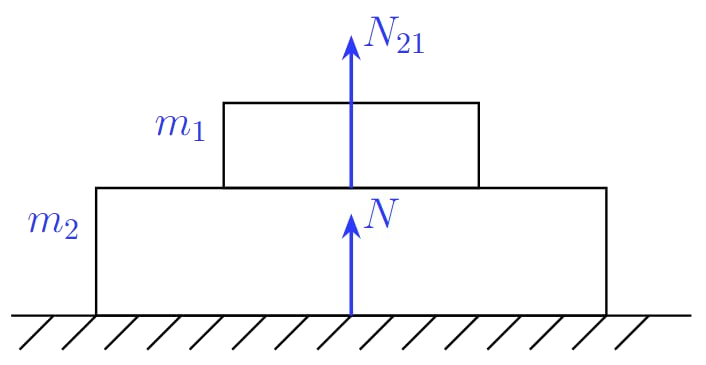
\includegraphics[width=0.33\linewidth]{7mgn.png}
\label{fig:mpr}
\end{center}


Если же слоистая система: два тела масс $m_1$ и $m_2$ одно на другом, и нижнее опирается на твердую плоскость, то
\[
N_{21} = m_1g,
\]

где $N_{21}$ — сила со стороны нижнего тела, действующая на верхнее, и
\[
N = (m_1 + m_2)g,
\]
где $N$ — реакция плоскости на нижнее тело. В общем случае при суммарной массе всех тел $m_{\rm сум}=\sum_i m_i$ реакция опоры равна
\[
N = m_{\rm сум}\,g.
\]

\textit{Вес тела} $P$ — это сила, с которой тело действует на опору, и по величине равна нормальной реакции опоры:
\[
P = N.
\]
Если тело покоится или движется равномерно по горизонтали, то нормальная реакция опоры уравновешивает силу тяжести $mg$, поэтому:
\[
P = N = mg.
\]

\end{document}